\documentclass[10pt]{article}
\usepackage[utf8]{inputenc}
\usepackage{listings}
\usepackage{float}
\usepackage{graphicx}
\usepackage{fullpage}
\usepackage{caption}
\usepackage{subcaption}
\usepackage{amsmath}
\usepackage{hyperref}
\usepackage{epstopdf}
\usepackage{csvsimple}

%\renewcommand{\thesubsection}{\arabic{subsection}}
\renewcommand{\thesubsubsection}{\alph{subsubsection}}

\title{Pattern Recognition Practical 6}
\author{Group 24: \and Maikel Withagen (s1867733) \and Steven Bosch (s1861948)}
\date{\today}
\lstset{
frame=single, 
numbers=left, 
breaklines=true, 
language=Matlab,
basicstyle=\footnotesize, 
title=\lstname,
showstringspaces=false
}

\DeclareMathOperator*{\argmax}{arg\!\max}

\renewcommand{\thesection}{Assignment \arabic{section}}
\renewcommand{\thesubsection}{\arabic{subsection}}
\begin{document}
\maketitle

\section{}
\subsection{}
The code in section \ref{Ass1} of the appendix was used to acquire the plots given in \ref{fig1.1}. As we can see, the sphering changes the signals in such a way that there is no dependency between them anymore.

\begin{figure}
  \centering
  \caption{The mixed signals before and after whitening.}
	\begin{subfigure}[b]{.49\textwidth}
		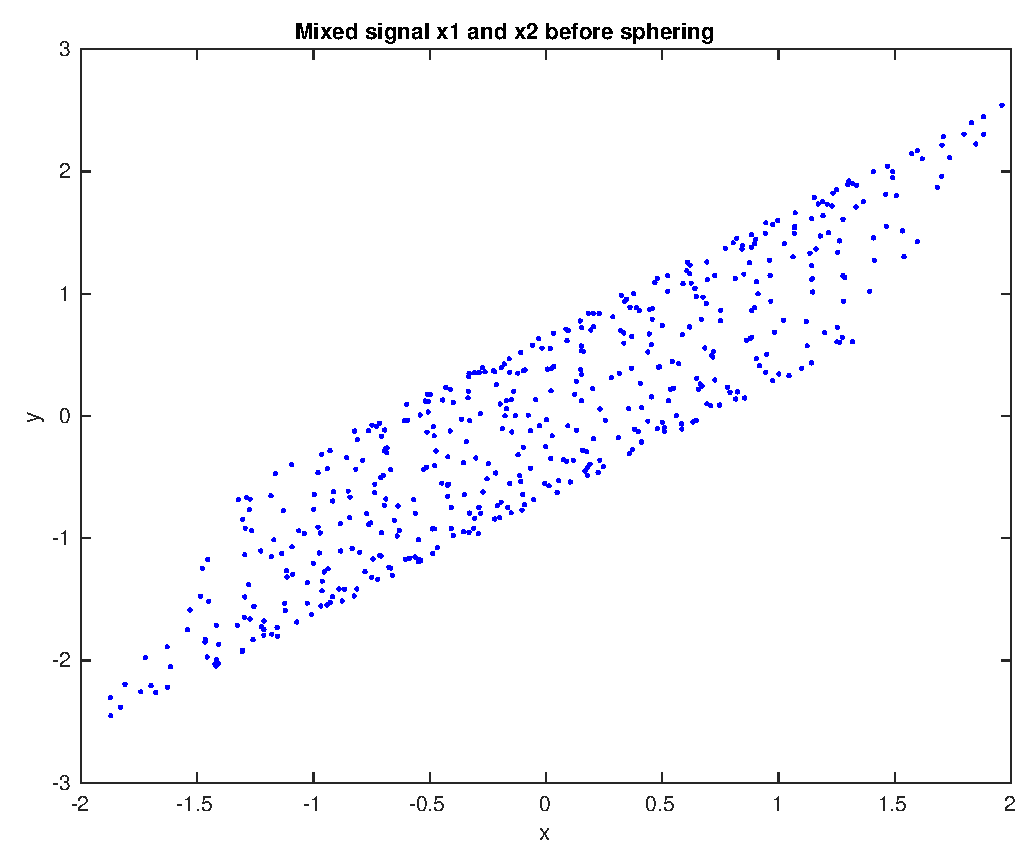
\includegraphics[width=\columnwidth]{Ass1a.eps}
		\caption{}
		\label{fig1a}
	\end{subfigure}  
	\begin{subfigure}[b]{.49\textwidth}
		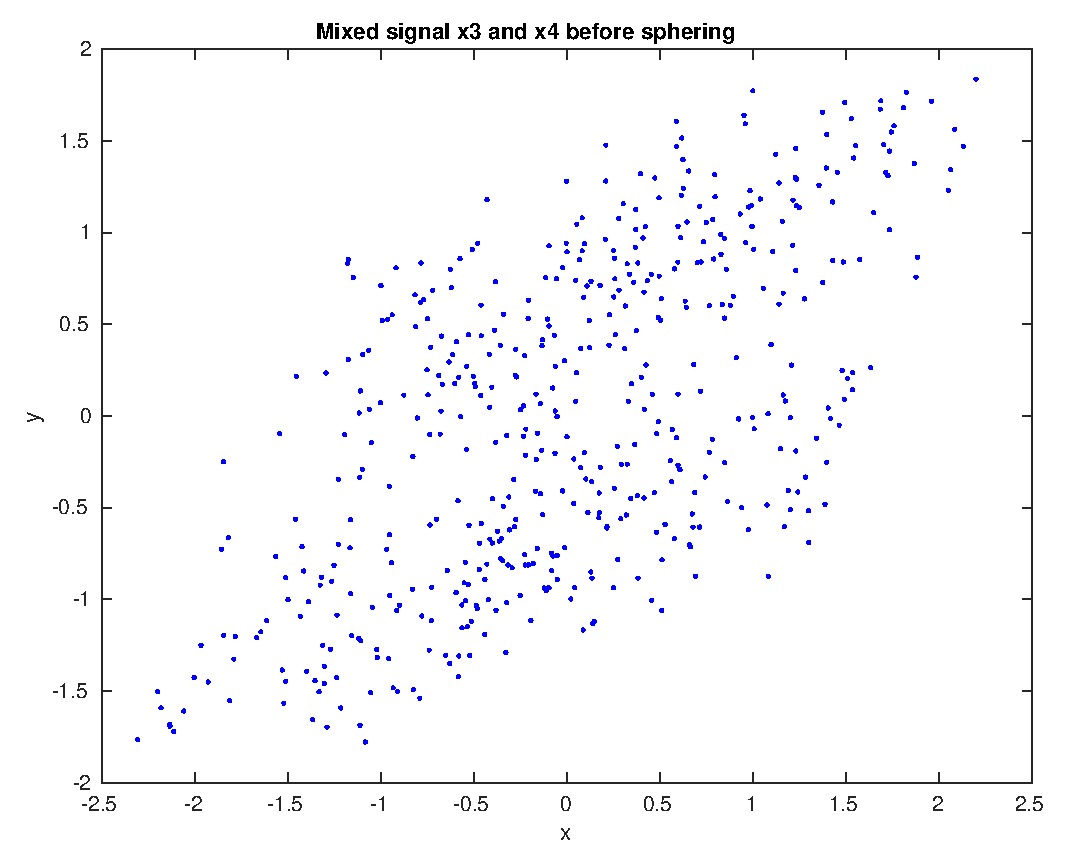
\includegraphics[width=\columnwidth]{Ass1b.eps}
		\caption{}
		\label{fig1b}
	\end{subfigure}
		\begin{subfigure}[b]{.49\textwidth}
		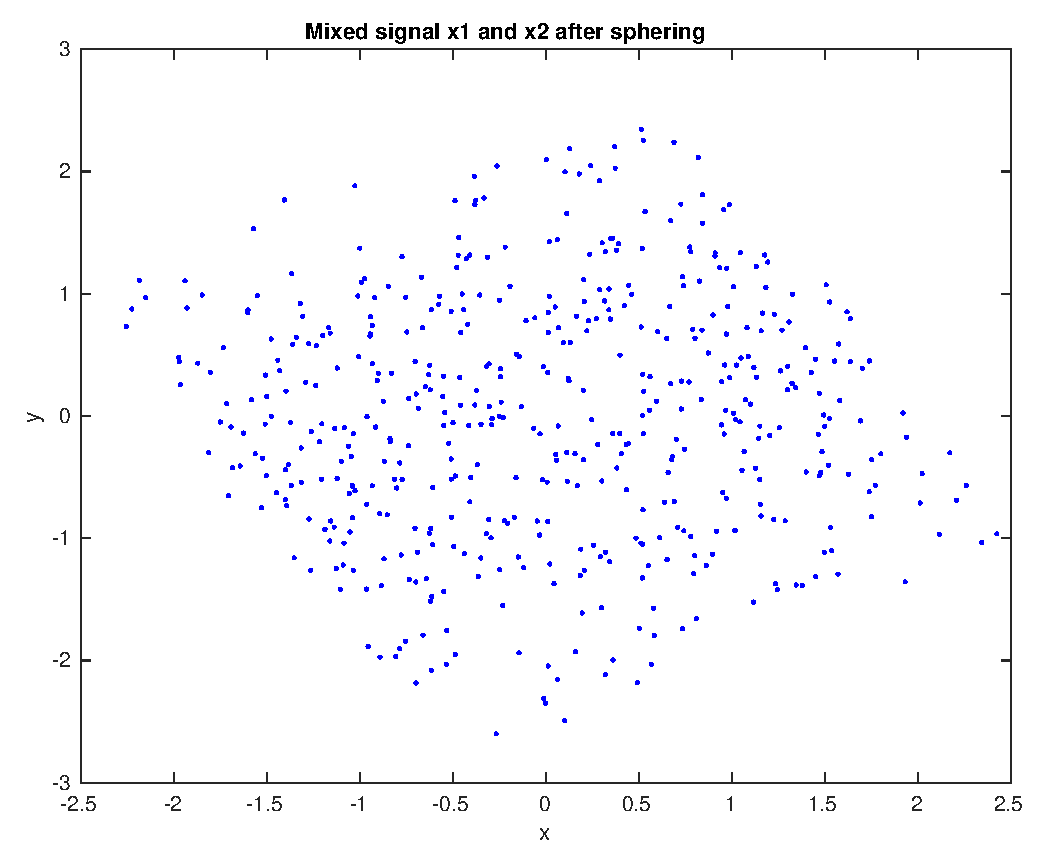
\includegraphics[width=\columnwidth]{Ass1c.eps}
		\caption{}
		\label{fig1c}
	\end{subfigure}  
	\begin{subfigure}[b]{.49\textwidth}
		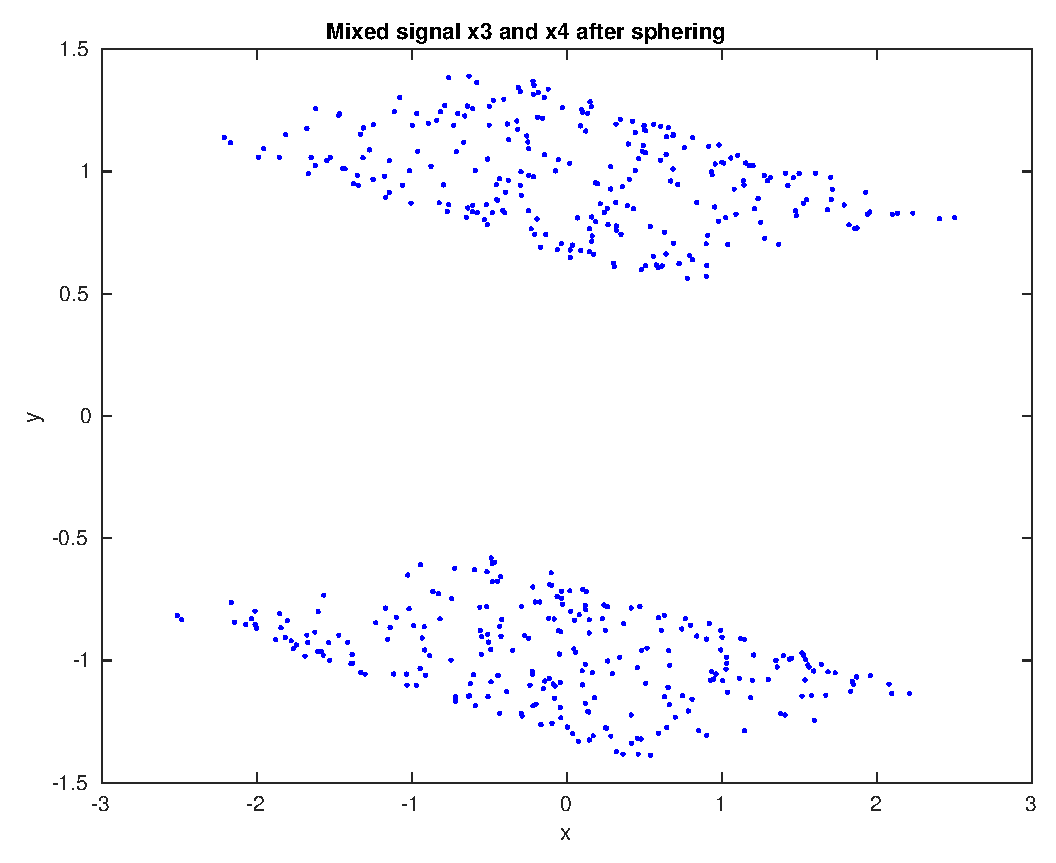
\includegraphics[width=\columnwidth]{Ass1d.eps}
		\caption{}
		\label{fig1d}
	\end{subfigure}
  \label{fig1.1}
\end{figure}

\subsection{}
The plots show that there is a clear correlation in unsphered signals (they seem to have a linear correlation, for every increase of x, there is an increase in y and vice versa), while the sphered signals do not have such relationships. In the plots of the sphered signals an increase in x does not necessarily lead to an increase or decrease in y (both are possible in either plot).
This is confirmed by the covariance matrices of the sphered signals:
\begin{lstlisting}
>> cov(spheredS(1,:), spheredS(2,:))

ans =

    1.0000    0.0000
    0.0000    1.0000

>> cov(spheredS(3,:), spheredS(4,:))

ans =

    1.0000    0.0000
    0.0000    1.0000
\end{lstlisting}
The covariance matrices are the identity matrices, indicating that there is no dependence between the signal vectors, since information about one signal does not give any information about the value of the other and vice versa (the corresponding covariance is 0).

\section{}
Our implementation of the fastICA is given in section \ref{Ass2} in the appendix.

\subsection{}

\subsection{}
The code given in section \ref{Ass2} in the appendix yields the plots given in figure \ref{fig2.1}.
\begin{figure}
  \centering
  \caption{The separate signals and the estimated independent component ($threshold = 0.0001, n = 1$.}
    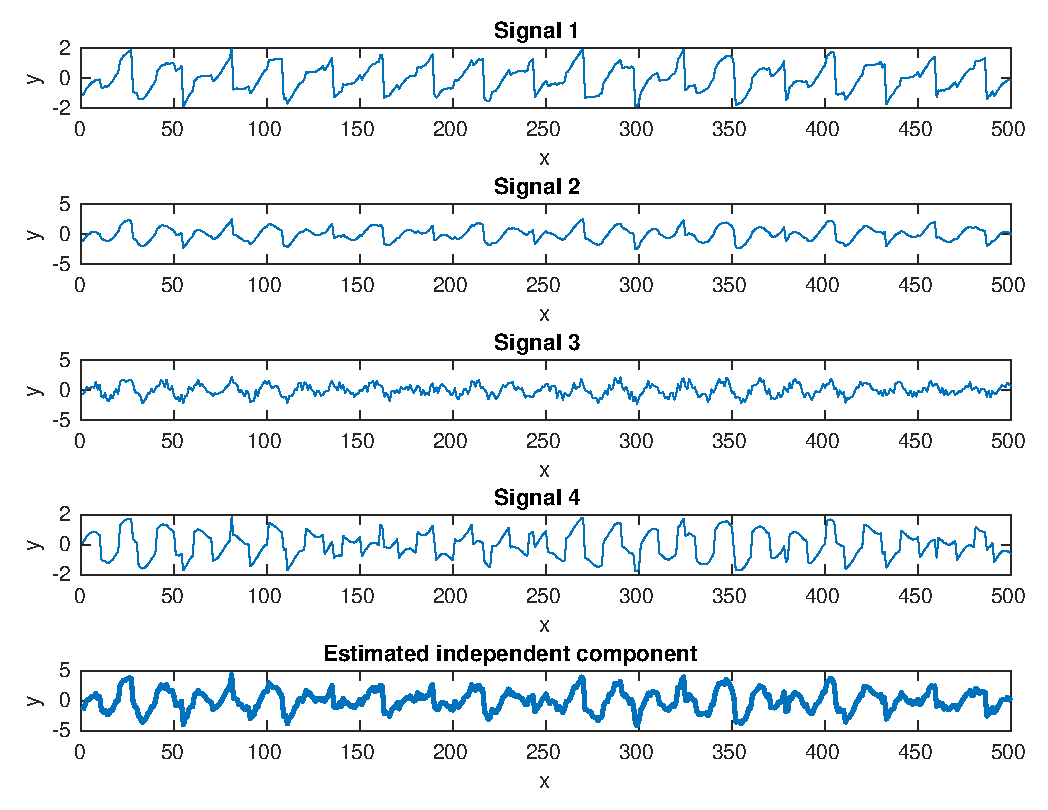
\includegraphics[width=\columnwidth]{Ass2.eps}
  \label{fig2.1}
\end{figure}
The plot shows that the estimated independent component is a combination of the four mixed signals that incorporates most of the variance of the four signals. As we can see it looks most like signal 4, suggesting that signal 4 resembles the most influental signal the most and shows the most variance out of the mixed signals.

\section{}

\newpage
\section*{Appendix}
\appendix
\section{Assignment 1}
\lstinputlisting{../Code/Ass1.m}{\label{Ass1}}
\section{Assignment 2 and 3}
\lstinputlisting{../Code/Ass1.m}{\label{Ass2}}

\end{document}
